\documentclass[a4paper,10pt]{report}

% Including essential packages for thesis formatting
\usepackage[utf8]{inputenc}
\usepackage[T1]{fontenc}
% \usepackage{libertinus}
\usepackage{lmodern}
\usepackage{float}[H]
\usepackage{tocloft}
\usepackage{amsmath}
\usepackage{graphicx}
\usepackage{geometry}
\usepackage{setspace}
\usepackage{booktabs}
\usepackage{hyperref}
\usepackage{enumitem}
\usepackage{natbib}


% Setting graphic path for images
\graphicspath{{./images/}}

% Configuring page geometry
\geometry{left=1.5in, right=1in, top=1in, bottom=1in}

% Setting up hyperlink styles
\hypersetup{
    colorlinks=true,
    linkcolor=black,
    filecolor=magenta,      
    urlcolor=cyan,
    citecolor=blue
}



% Customizing table of contents
\cftsetindents{chapter}{0em}{2em}
\cftsetindents{section}{2em}{3em}
\cftsetindents{subsection}{4em}{4em}
\setlength{\cftbeforechapskip}{0.5em}

% Defining document metadata
\title{Your Thesis Title}
\author{Loris Prataiolo}
\date{September 2025}


% Begin Document
\begin{document}

\begin{titlepage}
    \centering

    % University logo
    \vspace*{2cm} 
    
\includegraphics[width=0.6\textwidth]{images/universita-degli-studi-di-genova-logo-vector.png} % Replace with your logo file name
    \vspace{1cm}

    % University name
    {\Large \textbf{Università di Genova}\par}
    \vspace{0.5cm}

    % Department
    {\normalsize Università degli Studi di Genova\par}
    {\normalsize Dipartimento di Scienze Matematiche, Fisiche e Naturali del DIBRIS\par}
    \vspace{1cm}

    % Thesis title
    {\Large \textbf{Implementazione di una Pipeline di Machine Learning per l'Addestramento e il Confronto di Modelli di Object Detection su Kubeflow e MLflow basata su Faster R-CNN}\par}
    \vspace{1cm}

    % Course
    {\normalsize Corso di Laurea in Informatica\par}
    \vspace{2cm}

    % Candidate and Relatore
    \begin{tabular}{ll}
        \textbf{Candidato:} & \hspace{5cm}\textbf{Relatore:} \\
        Loris Prataiolo & \hspace{5cm}Prof.ssa Giovanna Guerrini \\
        & \\
        & \hspace{5cm}\textbf{Tutor Aziendale:} \\
        & \hspace{5cm}Dott. Luca Bianconi \\
    \end{tabular}
    \vspace{3cm}

    % Academic year
    {\normalsize Anno Accademico 2024/2025\par}

    \vspace*{\fill} 
\end{titlepage}

\newpage
\thispagestyle{empty}
\null{}
\newpage

\begin{abstract}
    La presente tesi si propone di mostrare la progettazione di una pipeline per l' addestramento di modelli di intelligenza artificale su Kubeflow in alternativa ad Apache Airflow, utilizzando come modello
    di base:  Faster R-CNN.\@ l' obbiettivo di questo lavoro, è la realizzazione di un sistema, robusto e adattabile a diversi contesti,
    in grado di poter gestire in autonomia l'intero ciclo di addestramento di un modello di AI.\@ 
    Il progetto è stato sviluppato su Google Cloud Platform (GCP), utilizzando come orchestratore il sistema Google Kubernates Engine (GKE), e Kubeflow per la realizzazione
    effettiva della pipeline.\@ Il risultato è un sistema versatile, in grado di supportare diversi modelli di AI, e diverse tipologie di dataset; mostrando l'efficacia di 
    di Kubeflow nel semplificare il ciclo di training di un modello, rispetto ad Airflow.\@
\end{abstract}

\newpage
\thispagestyle{empty}
\null{}
\newpage
\tableofcontents

\newpage
\thispagestyle{empty}
\null{}
\newpage

\chapter{Introduzione}
La presente tesi è frutto del lavoro svolto durante il tirocinio curricolare presso STAM Tech S.r.l.,
azienda Genovese operante nel settore IT, e attiva nello svilippo di tecnologie innovative a livello nazionale e internazionale.

\section{Contesto e obiettivi del progetto}

Il progetto è stato pensato per esplorare e implementare soluzioni innovative per l'integrazione di strumenti di pipelining AI alternativi ad Apache Airflow, con l'obiettivo di migliorare l'efficienza e la scalabilità
dei flussi di lavoro di machine learning.
Il cuore del progetto risiede nell'utilizzo di \textbf{KubeFlow},e del suo modulo \textbf{Pipelines} per l' escuzione e monitoraggio del processo di training dei modelli.
\\

Gli obiettivi principali del progetto includono:
\begin{itemize}
    \item Studio e comprensione delle funzionalità di KubeFlow e della sua integrazione con Kubernetes.
    \item Sviluppo di pipeline di machine learning utilizzando KubeFlow Pipelines, prendendo come base il modello Faster R-CNN.\@
    \item Studio dello strumento \textbf{MLFlow} come strumento di raccolta e monitoraggio delle metriche di training dei modelli.
    \item Valutazione dell' efficacia di KubeFlow rispetto ad Apache Airflow in termini di scalabilità, facilità d'uso e di come l' integrazione
    di MLFlow possa migliorare il monitoraggio dei modelli in fase di training.
\end{itemize}

Il lavoro svolto ha richiesto uno studio approfondito delle tecnologie coinvolte, nonchè una fase di sperimentazione pratica su come allenare un modello di object detection,
e uno studio di come monitorare le metriche di training in modo efficace.




\chapter{Tecnologie e Modelli Object Detection}
\section{Funzionamento ad alto livello dei modelli di AI per Object Detection}

I modelli di intelligenza artificiale di Object Detection sono progettati per
identificare e localizzare oggetti specifici all'interno di immagini o video. 
Questa classe di modelli combina tecniche di computer vision e deep learning per
analizzare il contenuto visivo e riconoscere pattern associati a diverse categorie
di oggetti.

Il processo di  \textit{Object Detection} generalmente consiste in due fasi:
\begin{itemize}
    \item \textbf{Rilevamento delle regioni di interesse (Region Proposal):} In questa fase, il modello identifica le aree dell'immagine che potrebbero contenere oggetti. Tecniche come Selective Search o Region Proposal Networks (RPN) sono comunemente utilizzate per generare queste proposte.
    
    \item \textbf{Classificazione e localizzazione:} Una volta identificate le aree di interesse, il modello classifica ciascuna regione in una delle categorie predefinite e determina la posizione esatta dell'oggetto all'interno della regione tramite le \textbf{bounding box}.
\end{itemize}


\subsection{Le Bounding Box}

Come accennato in precedenza, le boundig box sono dei rettangoli che vengono 
utilizzati per localizzare gli oggetti all'interno di un' immaagine, o di un frame
nel caso di un video.
Esse sono definite da quattro coordinate: (x\textsubscript{min}, y\textsubscript{min})
e (x\textsubscript{max}, y\textsubscript{max}), che rappresentano gli angoli superiore
sinistro e inferiore destro del rettangolo, rispettivamente. Ad ogni bounding box
viene associata anche una \textbf{classe} che identifica il tipo di oggetto
rappresentato (ad esempio, persona, auto, cane, ecc.) e una \textbf{confidenza}
che indica la probabilità che l'oggetto rilevato appartenga a quella classe.

\begin{figure}[H]
    \centering
    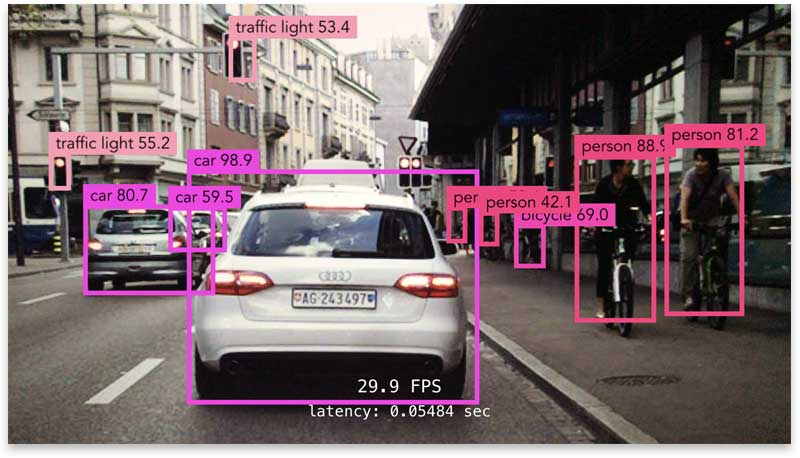
\includegraphics[width=0.5\textwidth]{images/car-bounding-boxes-sample.jpg}
        \caption{Un frame di una video camera, che mostra le vetture e semafori identificati da 
        bounding box, alle quali sono associati la classe e la confidenza.\\
        Fonte: \url{https://machinethink.net/blog/object-detection/}}
    \label{fig:bounding_box}
\end{figure}

Tuttavia, per motivi di semplicità e standardizzazione, le bounding box sono
solitamente definite all'interno di un file di annotazione associato all'immagine.
La struttura tipica di un dataset per l'addestramento e il test di modelli di Object Detection
viene rappresentato nel seguente modo:

\begin{figure}[H]
    \centering
    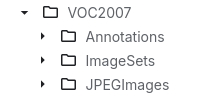
\includegraphics[width=0.5\textwidth]{images/OD-dataset-sample-pascal-voc-07.png}
        \caption{Esempio struttura tipica di un dataset per l'addestramento e il test di modelli di Object Detection, attraverso PASCAL VOC 2007.\\
        Fonte: \url{https://www.kaggle.com/datasets/zaraks/pascal-voc-2007}}
    \label{fig:dataset_structure}

\end{figure}

Una nota che vale la pena sottolineare ora ma che verrà approfondita più in avanti, è che il dataset non viene dato in pasto al modello
così com'è, perchè ogni modello, a seconda della sua architettura, richiede che i dati
siano formattati in un certo modo. Per questo motivo, prima di essere utilizzato per
l'addestramento, il dataset deve essere \textbf{preprocessato} per adattarsi ai requisiti specifici del modello scelto.


\subsection{L'importanza del dataset}
Il dataset in un contesto di Object Detection è un aspetto cruciale per il successo
dell'addestramento di un modello focalizzato su questo specifico compito.
Il dataset non deve avere solo una quantità sufficente di immagini per ogni classe,
ma deve essere anche il più vario e ampio possibile, permettendo al modello di
imparare a riconoscere gli oggetti in diverse condizioni.
Infatti il riconoscimento di oggetti viene influenzato da molteplici fattori, tra cui:

\begin{itemize}
    \item \textbf{Angolazione e prospettiva:} Una delle difficoltà 
    principali nell'addestramento di modelli di Object Detection è la variazione
    della prospettiva da cui un oggeetto può essere visto. Variando l'Angolazione
    cilindro può apparire come un cerchio, un ovale o un rettangolo, a seconda
    dell'angolazione da cui viene osservato.

    \item \textbf{Illuminazione e condizioni ambientali:} L'illuminazione ha una grande
    influenza sulla definizione e visibilità degli oggetti. Anche in questo caso,
    un oggetto può apparire molto diverso in condizioni di luce intensa rispetto
    a condizioni di scarsa illuminazione. Inoltre, condizioni atmosferiche come
    pioggia, nebbia o neve possono ulteriormente complicare il riconoscimento
    degli oggetti.

    \item \textbf{Occlusione:} Gli oggetti possono risultare parzialmente nascosti da altri oggetti
    o elementi nell'ambiente. Questo fenomeno,  rappresenta una  sfida significativa
    per i modelli di Object Detection, poichè devono essere in grado di identificare
    gli oggetti anche quando non sono completamente visibili.

\end{itemize}

\subsection{Suddivisione del dataset}

La fase di addestramento la si analizzerà più avanti, durante la fase implementativa del progetto,
ma è importante sottolineare che il dataset viene solitamente pensato per essere suddiviso in tre sottoinsiemi distinti:
\begin{itemize}
    \item \textbf{Training set:} Utilizzato per addestrare il modello
    \item   \textbf{Validation set:} Utilizzato per ottimizzare i parametri del modello
    \item \textbf{Test set:} Utilizzato per valutare le prestazioni finali del modello
\end{itemize}

\subsection{Modello Faster R-CNN}
Basato su R-CNN (Region-based Convolutional Neural Networks), il Faster R-CNN è un modello di Object 
Detection il cui scopo è quello di poter rilevare oggetti in immagini e video in modo rapido ed efficiente.
Il miglioramento significativo approtato al modello precedente è stata la Region Proposal Network, RPN,
o in italiano Rete di \textit{Proposta delle Regioni}, che consente al modello di generare proposte di regioni in modo molto più veloce
rispetto ai metodi precedenti.\\

\subsubsection{La Region Proposal Network (RPN)}
La \textit{RPN} è una rete neurale convoluzionale che scansiona l'immagine di input e propone
regioni che potrebbero contenere oggetti. Queste regioni vengono poi passate alla fase di classificazione
e localizzazione. La fase di classificazione determina la probabilità che una regione contenga 
l' oggetto di interessse. La fase di localizzazione, invece, inferisce le coordinate della regione proposta.

\subsubsection{Visone d'insieme dell'architettura di Faster R-CNN}

\begin{figure}[H]
    \centering
    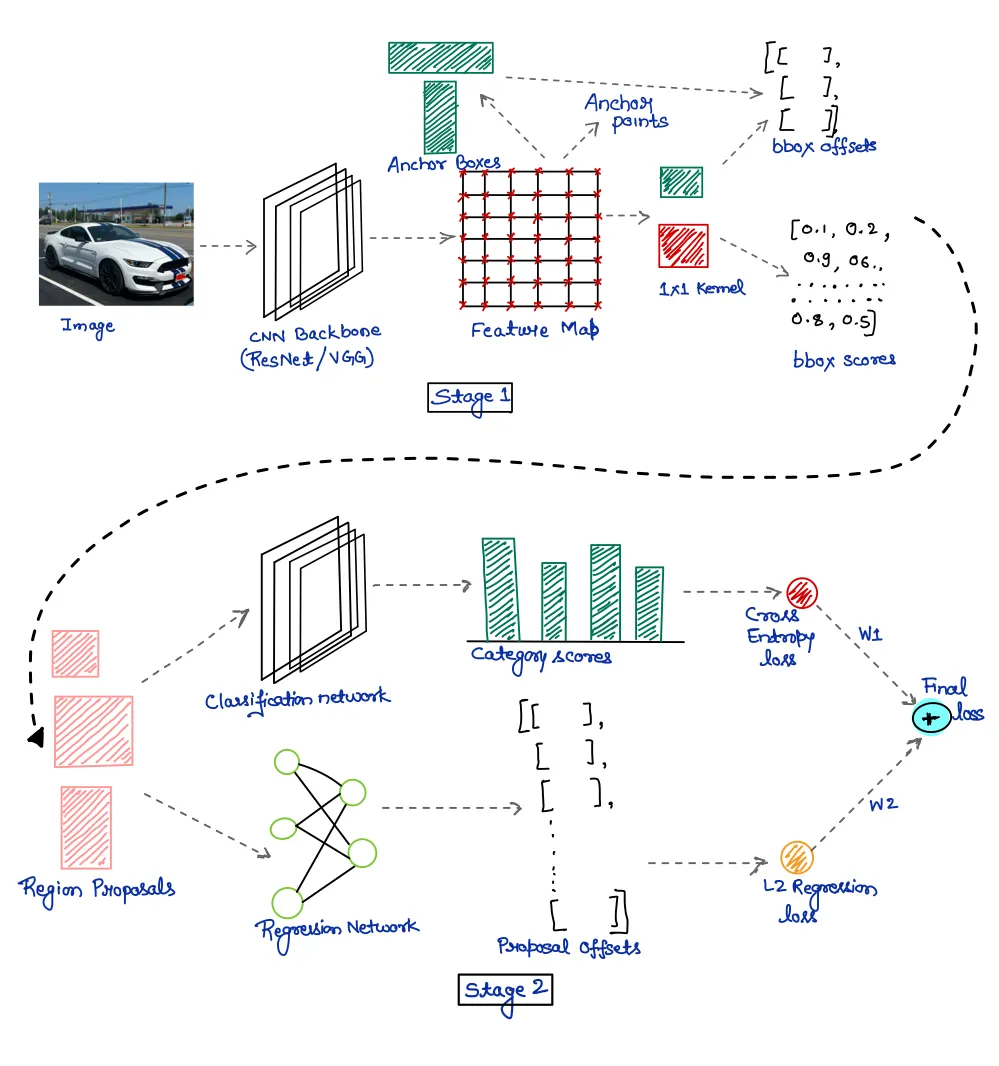
\includegraphics[width=0.5\textwidth]{images/faster_rcnn_architecture.png}
        \caption{Architettura di Faster R-CNN.\\
        Fonte: \url{https://medium.com/@RobuRishabh/understanding-and-implementing-faster-r-cnn-248f7b25ff96}}
    \label{fig:faster-rcnn-architecture}
\end{figure}

Come mostrato in figura \ref{fig:faster-rcnn-architecture}, l'architettura di Faster R-CNN 
è composta da due fasi principali:\\

\textbf{1. Region Proposal Network}
L' immagine viene analizzata da una rete neurale convoluzionale (CNN) per estrarre
le caratteristiche rilevanti dell'immagine. Da queste caratteristiche, il blackbone
genera la mappa delle caratteristiche (feature map). La RPN scansiona questa mappa 
e identifica le regioni che potrebbero contenere gli oggetti.Per ogni regione proposta,
la RPN calcola due valori principali: la probabilità che la regione contenga un oggetto
e le coordinate della bounding box che delimita l'oggetto. Queste ultime, se la probabilità
è sufficentemente alta, vengono rifinite e passate alla fase successiva.\\

\textbf{2. Fase di classificazione e localizzazione}
Le regioni proposte le quali auspicabilmente contengono gli oggetti di interessi,
vengono rielaborate e rifinite da una seconda rete convoluzionale: la \textbf{RoI Pooling Layer}.
Questa rete adatta le regioni proposte a una dimensione fissa, rendendole compatibili
con la rete di classificazione. Successivamente, le regioni vengono passate a una rete
neurale completamente connessa (fully connected), che esegue la classificazione e la
localizzazione finale. La rete assegna una classe a ciascuna regione e regola ulteriormente
le coordinate della bounding box per migliorare la precisione della localizzazione.




\section{Kubernates e Kubeflow}
\begin{figure}[H]
    \centering
    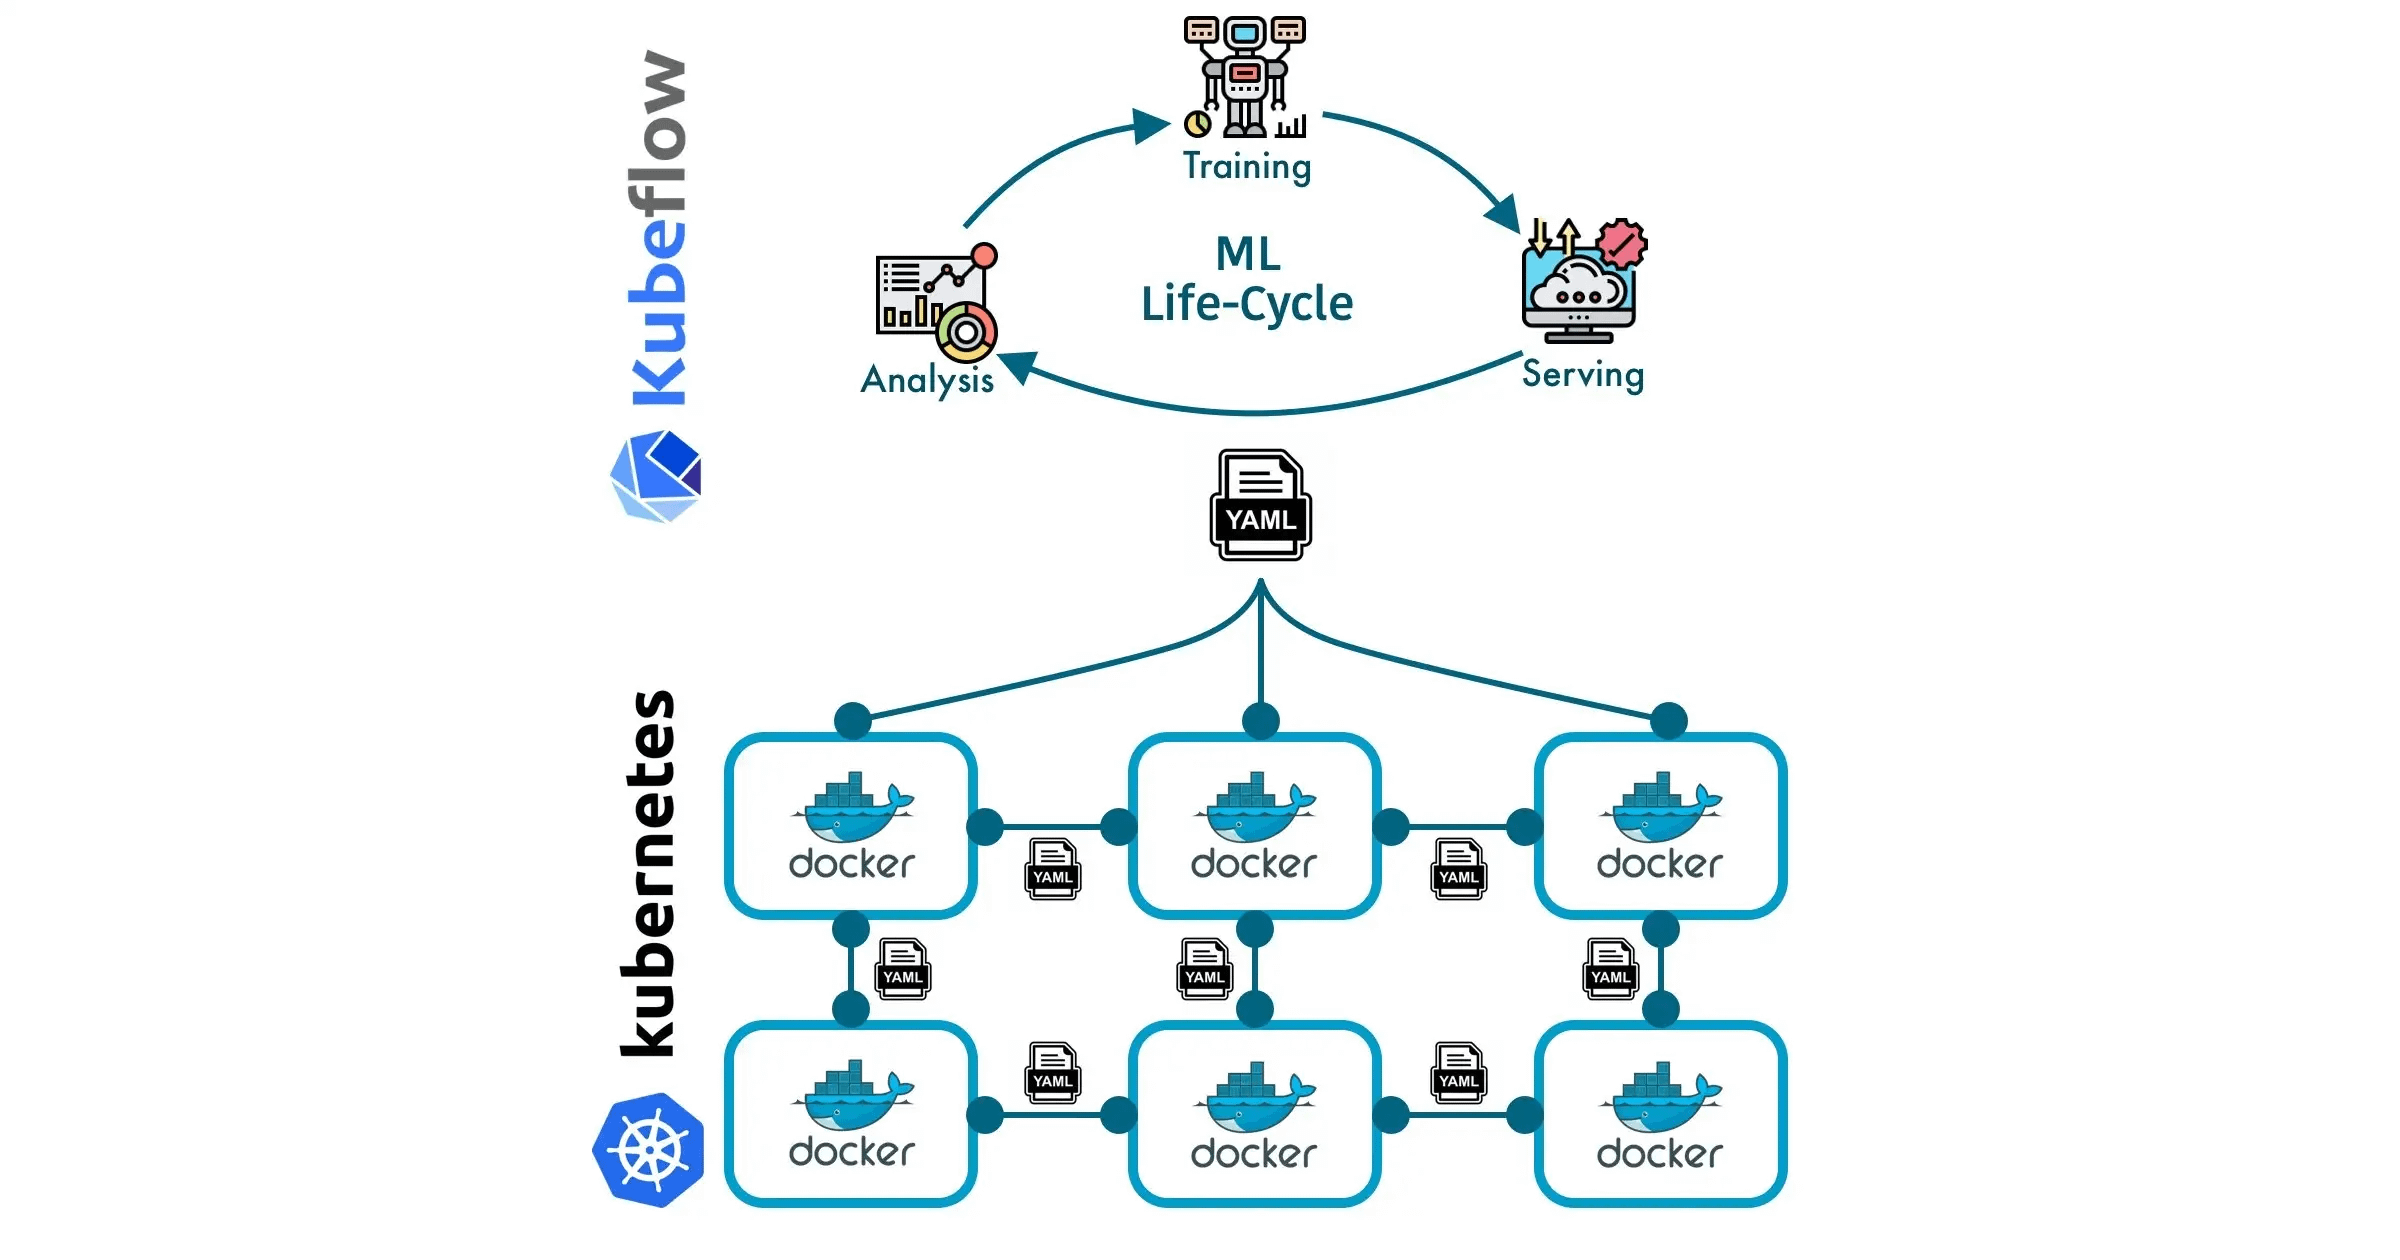
\includegraphics[width=0.7\textwidth]{images/kubernates-kubeflow-schema.png}
        \caption{Schema architetturale di come Kubeflow e Kubernates operano tra di loro.\\
        Fonte: \url{https://www.reddit.com/r/kubernetes/comments/zxddtv/fastkubeflow_kubeflow_tutorial_sample_usage/}}
    \label{fig:kubeflow-architecture}
\end{figure}

La collaborazione tra Kubeflow e Kubernetes verrà, qui di seguito  analizzata utilizzando
un'approccio top-down, partendo da Kubeflow e scendendo fino a Kubernetes.\\

\subsection{Kubeflow}
Kubeflow è una piattaforma open-source progettata per fornire un ambiente completo
per lo sviluppo, l'addestramento e il deployment di modelli di machine learning (ML)
su Kubernetes. L'obiettivo principale di Kubeflow è quello di semplificare il processo
di gestione del ciclo di vita dei modelli di ML, consentendo agli sviluppatori
di concentrarsi sulla creazione di modelli piuttosto che sulla gestione dell'infrastruttura.\\

\clearpage
\subsubsection{Panoramica delle componenti principali di Kubeflow}
\begin{figure}[H]
    \centering
    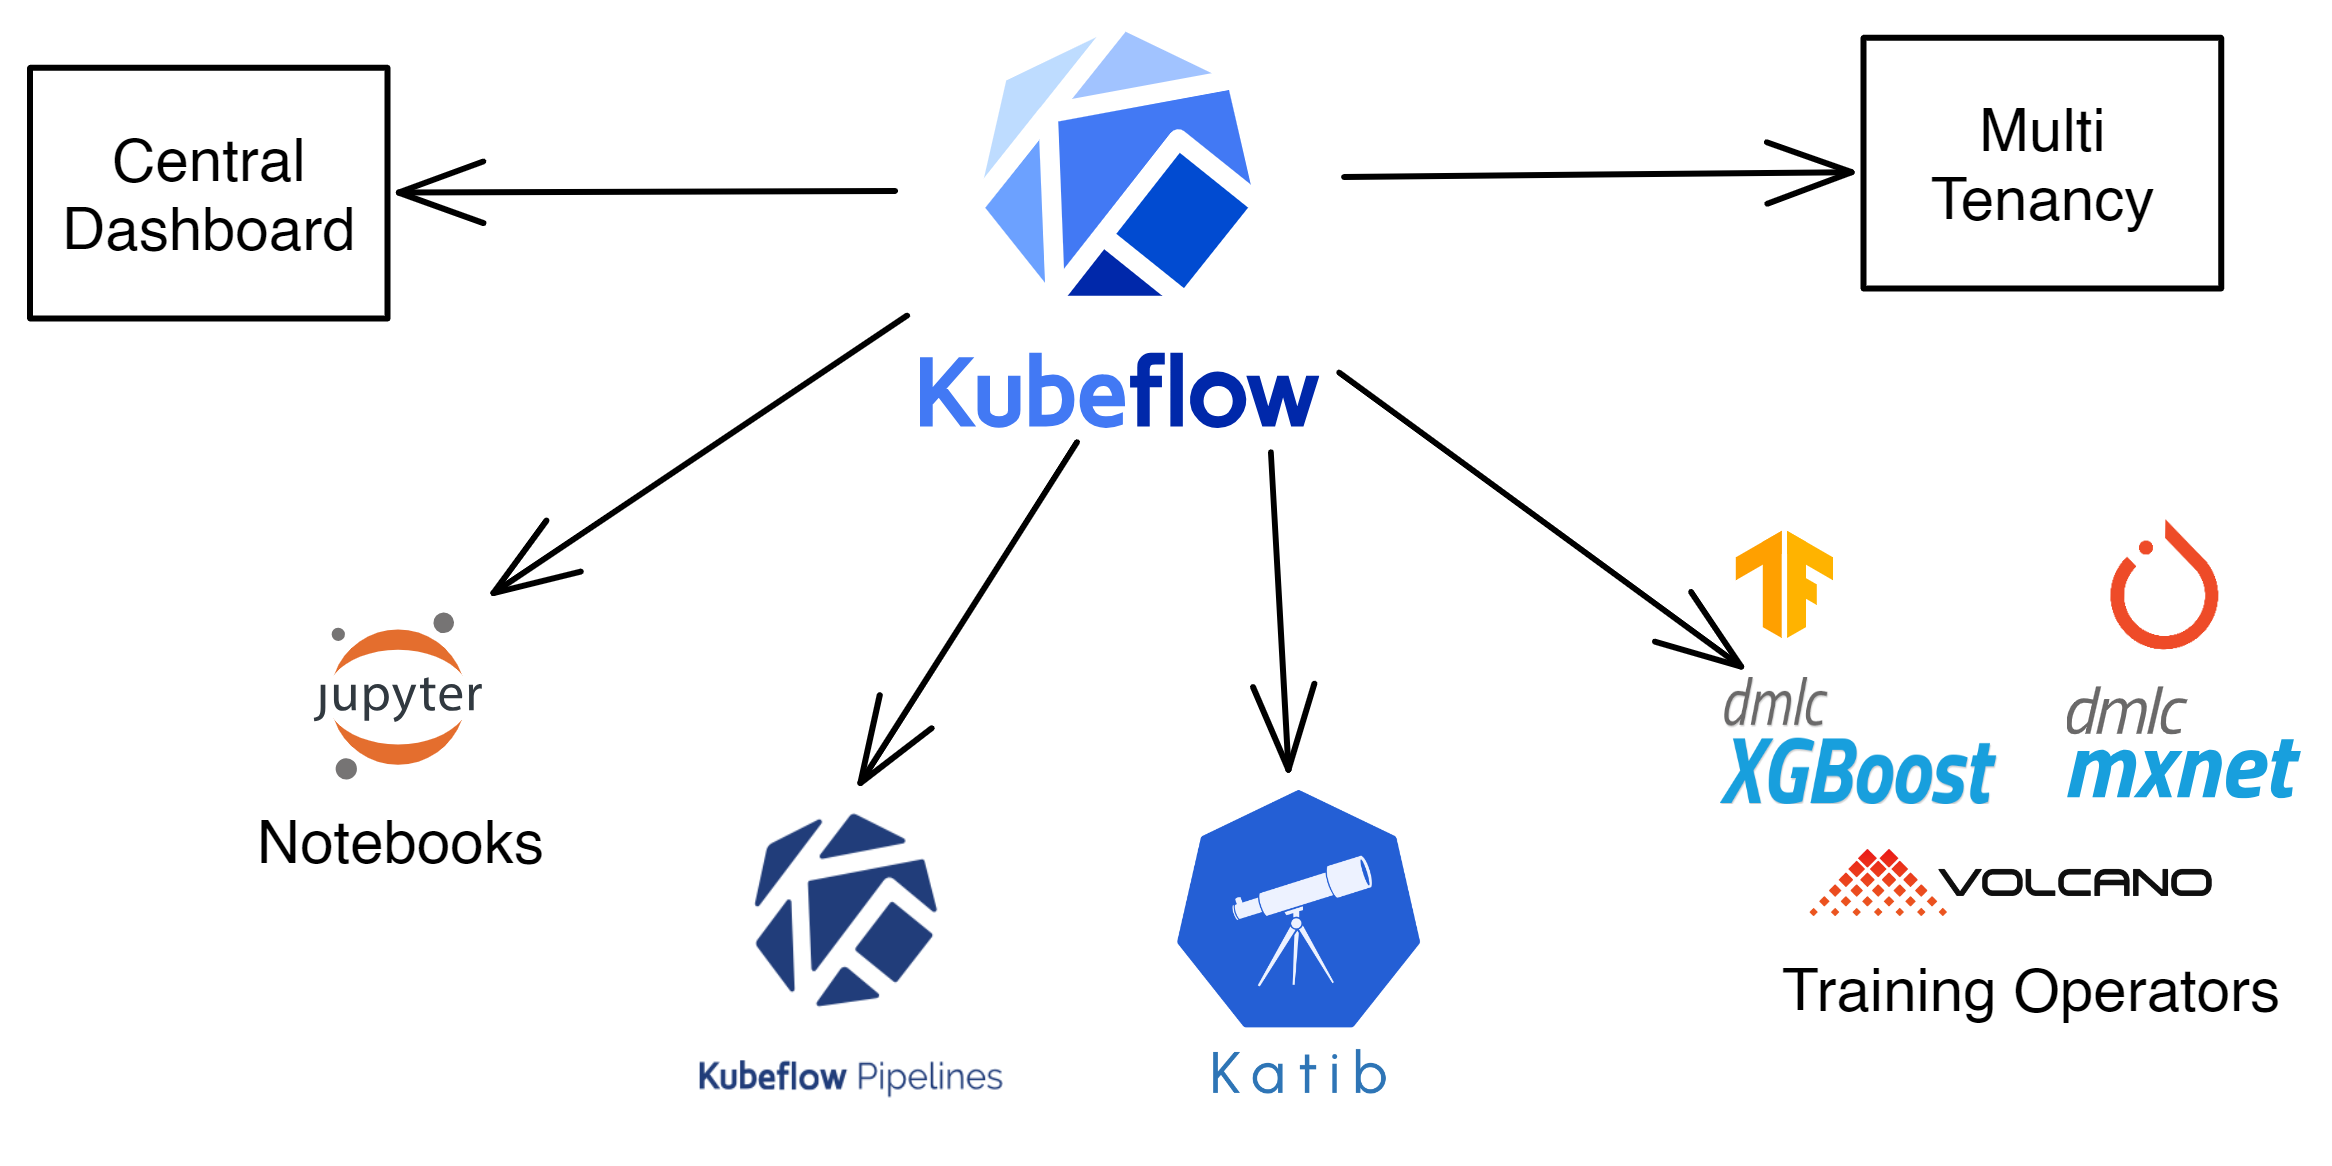
\includegraphics[width=0.7\textwidth]{images/kubeflow-components.png}
        \caption{Componenti principali di Kubeflow.\\
        Fonte: \url{https://www.biaodianfu.com/kubeflow.html}}
    \label{fig:kubeflow-components}
\end{figure}

Come mostrato in figura \ref{fig:kubeflow-components}, Kubeflow è composto da diverse
componenti principali. Questi moduli possono essere utilizzati singolarmente o in combinazione
per creare flussi di lavoro di machine learning complessi. Le componenti principali includono:
\begin{itemize}
    \item \textbf{Kubeflow Pipelines:} Un sistema per la creazione, l'esecuzione e la gestione
    di flussi di lavoro di machine learning. Verrà approfondito poco più sotto.
    \item \textbf{Katib:} Un sistema di ottimizzazione automatica dei parametri (hyperparameter tuning)
    che aiuta a migliorare le prestazioni dei modelli di ML.\@
    \item \textbf{KFServing:} Una piattaforma per il deployment e la gestione di modelli di ML
    in produzione. Nel contesto del progetto in esame, questa componente avrebbe permesso al modello
    di essere esposto come servizio web, consentendo l'inferenza in tempo reale.
    \item \textbf{Jupyter Notebooks:} Un ambiente di sviluppo che consente di poter definire il codice
    direttamente all'interno del sistema di kubeflow.Questa componente consente di poter scegliere tra diversi
    enviroment: Colab, VsCode, e Jupyter. Tuttavia, è bene notare che questa componente
    non è stata utilizzata nel progetto in esame a causa di limitazione di risorse, le quali verranno
    discusse più avanti.
\end{itemize}


\subsubsection{Kubeflow Pipelines}
\textit{Kubeflow Pipelines} è la componente \textit{core} di questo progetto di tesi, 
pertanto merita un'analisi più approfondita.\\

Una pipeline di machine learning è una serie di passaggi sequenziali i quali vengono
progettati per automatizzare il processo di processamento dei dati, l'addestramento del modello
e la valutazione delle prestazioni. Le pipeline consentono di standardizzare e ripetere
questi processi, migliorando l'efficienza e la coerenza dei risultati.

\begin{figure}[H]
    \centering
    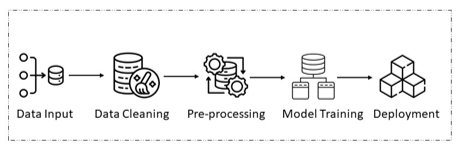
\includegraphics[width=0.7\textwidth]{images/overview-ml-pipeline-structure.jpg}
        \caption{Struttura base di una pipeline di machine learning.\\
        Fonte: \url{https://www.design-reuse.com/article/61411-an-overview-of-machine-learning-pipeline-and-its-importance/}}
    \label{fig:ml-pipeline-structure}
\end{figure}

Il modulo di Kubeflow, non permette di creare direttamente la pipeline. La pipeline,
viene definita attraverso un codice Python, utilizzando
il \textbf{Software Developer Kit} (SDK) di Kubeflow. Una volta definita, ed elaborata attraverso l'SDK, viene generato
un file in formato \textbf{YAML}, il quale viene poi caricato all'interno di Kubeflow
attraverso l'interfaccia grafica, e a quel punto \textit{Kubeflow Pipelines} inferisce
la struttra della pipeline e la rende eseguibile. Difatto, questo modulo
si occupa di  eseguire la pipeline, gestendo le varie componenti della pipeline 
nel modo più efficente possibile.\\

Ogni componente, all'interno del codice, viene definito come una funzione. Tuttavia,
per essere riconosciuta come componente di una pipeline, la funzione deve essere
decorata con un apposito decoratore fornito dall'SDK di Kubeflow.
Inoltre, deve rispettare alcune regole specifiche, come l'uso di tipi di dati supportati
e la gestione degli input e output in modo appropriato. Ma la caratteristica più importante
è che ogni componente deve essere concepito come un programma indipendente, il quale
può essere eseguito in isolamento. Questo significa che ogni componente deve essere in grado
di eseguire il proprio compito senza dipendere da altre parti del codice.\\

Questo è dovuto alla natura distributiva di Kubeflow e di ciò che lo sorregge: Kubernetes.
Difatti, ogni componente viene eseguito all'interno di un \textbf{pod} di Kubernetes.
Un pod è la più piccola unità eseguibile che può essere creata e gestita in Kubernetes.
Un pod può contenere uno o più container, i quali condividono le risorse di rete e di storage.
Ogni pod viene eseguito su un nodo del cluster di Kubernetes, il quale può essere una macchina fisica
o virtuale.\\

Anche in questo caso, possiamo vedere come Kubeflow sia estremamente comodo per l'utente,
infatti, tutte queste complessità vengono gestite in modo automatico da Kubeflow. Quello che 
un programmatore deve fare, è definire le componenti della pipeline come funzioni, ma rispettando
le regole sopra menzionate. Una volta caricata la pipeline e avviata, kubefow si occuperà
di creare i pod necessari per eseguire ogni componente, gestendo la distribuzione e la scalabilità
in modo trasparente per l'utente.


\subsection{Kubernetes e il ruolo nelle pipeline di Kubeflow}
Kubernetes è una piattaforma open-source per l'orchestrazione di container, che consente
di automatizzare il deployment, la scalabilità e la gestione delle applicazioni containerizzate.
Anche se kubernates è open-source, è estremamente complesso da utilizzare e gestire.
Per questo motivo, molte aziende scelgono di utilizzare servizi gestiti come Google Kubernetes Engine (GKE),
Amazon Elastic Kubernetes Service (EKS) o Azure Kubernetes Service (AKS).\\

Come accennato in precedenza, ogni componente di una pipeline
deve essere concepito come un programma indipendente, il quale
può essere eseguito in isolamento.
Questo è dovuto alla natura di come Kubeflow opera, infatti,
all'esecuzione di una pipeline, per ogni componente viene creato
un pod di Kubernetes. Ogni pod viene eseguito su un nodo del cluster di Kubernetes
il quale può essere una macchina fisica o virtuale.
Una volta che il pod ha completato il suo compito, viene terminato, e
il prodotto viene passato all'eventuale pod successivo.\\

Anche se Kubeflow e Kubernates si occupano della gestione dei pod,
è stato fondamentale avere una conoscenza di come kubernates opera, siccome
come si discuterà più avanti, i pod possono anche fallire,
e in quel caso, è stato necessario intervenire manualmente
per risolvere il problema.







% Bibliography
~\cite{*}
\bibliographystyle{plainnat}
\bibliography{capitoli/references}
\end{document}


